\documentclass[a4paper,14pt]{extarticle}

\usepackage[utf8x]{inputenc}
\usepackage[T1,T2A]{fontenc}
\usepackage[russian]{babel}
\usepackage{hyperref}
\usepackage{indentfirst}
\usepackage{here}
\usepackage{array}
\usepackage{graphicx}
\usepackage{caption}
\usepackage{subcaption}
\usepackage{chngcntr}
\usepackage{amsmath}
\usepackage{amssymb}
\usepackage{pgfplots}
\usepackage{pgfplotstable}
\usepackage[left=2cm,right=2cm,top=2cm,bottom=2cm,bindingoffset=0cm]{geometry}
\usepackage{multicol}

\renewcommand{\le}{\ensuremath{\leqslant}}
\renewcommand{\leq}{\ensuremath{\leqslant}}
\renewcommand{\ge}{\ensuremath{\geqslant}}
\renewcommand{\geq}{\ensuremath{\geqslant}}
\renewcommand{\epsilon}{\ensuremath{\varepsilon}}
\renewcommand{\phi}{\ensuremath{\varphi}}

\counterwithin{figure}{section}
\counterwithin{equation}{section}
\counterwithin{table}{section}
\newcommand{\sign}[1][5cm]{\makebox[#1]{\hrulefill}} % Поля подписи и даты
\graphicspath{{pics/}} % Путь до папки с картинками
\captionsetup{justification=centering,margin=1cm}
\def\arraystretch{1.3}

\begin{document}

\begin{titlepage}
\begin{center}
	\textbf{Санкт-Петербургский Политехнический Университет \\Петра Великого}\\[0.3cm]
	\small Институт компьютерных наук и технологий \\[0.3cm]
	\small Кафедра компьютерных систем и программных технологий\\[4cm]
	
	\textbf{ОТЧЕТ}\\ \textbf{о лабораторной работе}\\[0.5cm]
	\textbf{<<Исследование частотных характеристик пассивных RC-цепей>>}\\[0.1cm]
	\textbf{Электротехника и Электроника}\\[10.5cm]
\end{center}

\begin{flushright}
	\begin{minipage}{0.60\textwidth}
		\begin{flushleft}
			\small \textbf{Работу выполнили студенты}\\[3mm]
			\small группа 23501/4 \hspace*{17mm} Дьячков В.В.\\[3mm]
			\small группа 23501/4 \hspace*{17mm} Ламтев А.Ю.\\[5mm]
			
			\small \textbf{Преподаватель}\\[5mm]
		 	\small \sign[3.5cm] \hspace*{8mm} к.т.н., доц. Кочетков Ю.Д.\\[0.5cm]
		\end{flushleft}
	\end{minipage}
\end{flushright}

\vfill

\begin{center}
	\small Санкт-Петербург\\
	\small \the\year
\end{center}
\end{titlepage}

\section{Цель работы}

Исследовать экспериментально переходные процессы, происходящие в транзисторном ключе.

\section{Чертеж схемы исследуемого устройства}

\begin{figure}[H]
	\begin{center}
	\vspace{-0.5cm}
		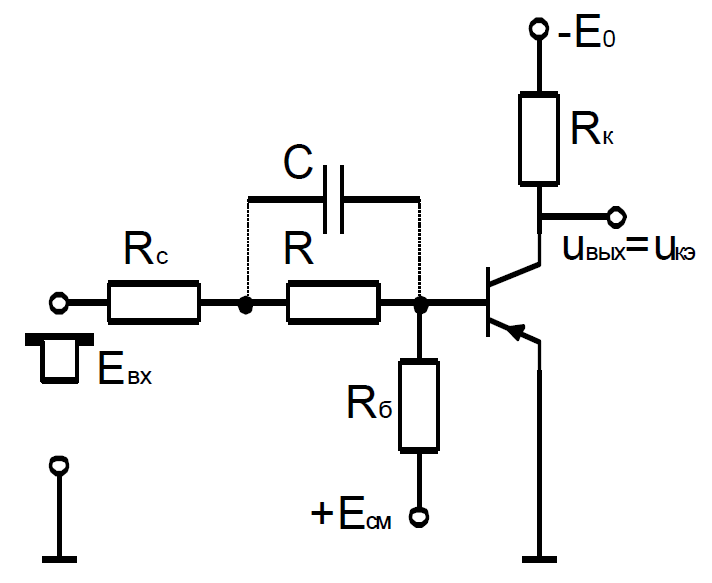
\includegraphics[width=7cm]{img/scheme}
		\caption{Схема транзисторного ключа с общим эмиттером}
		\label{figure:1}
	\vspace{-0.5cm}
	\end{center}
\end{figure}

\section{Исходные данные}

Транзистор МП25. Германиевый транзистор с $p-n-p$ переходом.

\begin{table}[H]
	\begin{center}
	\caption{Исходные данные}
	\def\arraystretch{1.4}
		\begin{tabularx}{\textwidth}{|X|X|X|X|X|X|X|X|X|X|}
			\hline
			$E_0$ &
			$E_\text{см}$ &
			$I_\text{кн}$ &
			$S$ &
			$E_\text{вх}$ &
			$t_\text{и}$ &
			$R_c$ &
			$I_{\text{к}_0\ \ max}$ &
			$B$ &
			$f_\alpha$\\
			\hline
			В &
			В &
			мА &
			 &
			В &
			мкс &
			кОм &
			мкА &
			 &
			кГц\\
			\hline
			25 &
			5 &
			20 &
			3 &
			7 &
			10 &
			1 &
			75 &
			19 &
			250 \\
		    \hline	
		\end{tabularx}
		\label{tabular:1}
	\end{center}
\end{table}

\section{Теоретические расчёты}

\subsection{Расчёт элементов цепи}

\begin{displaymath}
R_\text{б} \leq \frac{E_0}{I_{\text{к}_0\ \ max}} = \frac{25}{75 \cdot 10^{-6}} = 330\ \ \text{кОм}
\end{displaymath}

\begin{displaymath}
R_\text{к} = \frac{E_0}{I_\text{кн}} = \frac{25}{20 \cdot 10^{-3}} = 1.25\ \ \text{кОм}
\end{displaymath}

\begin{displaymath}
I_{\text{б}_1} = \frac{S \cdot I_\text{кн}}{B} = \frac{3 \cdot 20 \cdot 10^{-3}}{19} = 3.16\ \ \text{мА}
\end{displaymath}

\begin{displaymath}
R = \frac{E_\text{вх}}{I_{\text{б}_1} + \frac{E_\text{см}}{R_\text{б}}} - R_\text{c} = \frac{7}{3.16 \cdot 10^{-3} + \frac{5}{330 \cdot 10^3}} - 1 = 1.2\ \ \text{кОм}
\end{displaymath}

\begin{displaymath}
\tau_{\text{б}} = \frac{B}{2 \cdot \pi \cdot f_\alpha} = \frac{19}{2 \cdot \pi \cdot 250 \cdot 10^3} = 1.21 \cdot 10^{-5}
\end{displaymath}\\[1cm]

\begin{displaymath}
I_{\text{б}_2} \simeq \frac{E_\text{см}}{R_\text{б}} = \frac{5}{330 \cdot 10^3} = 1.51 \cdot 10^{-5}\ \ \text{A}
\end{displaymath}

\begin{displaymath}
d = \frac{I_{\text{б}_2}}{I_{\text{б}_1}} = \frac{ 1.51 \cdot 10^{-5}}{3.16 \cdot 10^{-3}} = 4.78 \cdot 10^{-3}
\end{displaymath}

\begin{displaymath}
C = \frac{\tau_{\text{б}}}{R \cdot \Big ( 1 + \frac{dR}{R+R_c} \Big )} = \frac{1.21 \cdot 10^{-5}}{1.2 \cdot 10^3 \cdot \Big ( 1 + \frac{4.78 \cdot 10^{-3} \cdot 1.2 \cdot 10^3}{1.2 \cdot 10^3+1000} \Big )} = 10 \text{нФ}
\end{displaymath}

\subsection{Расчёт $t_\text{ф}$, $t_\text{сп}$, $t_\text{расс}$}

\begin{equation}
\label{t_f}
t_\phi = \tau_{\text{б}} \cdot \ln{\frac{I_{\text{б}_1}}{I_{\text{б}_1} - 0.9 \cdot \frac{I_\text{кн}}{B}}}
\end{equation}

$I_{\text{б}_2} = 1.51 \cdot 10^{-5} \ll \frac{I_\text{кн}}{B} = \frac{20}{19} \Rightarrow$
\begin{equation}
\label{t_sp}
t_\text{сп} = 2.3 \cdot \tau_\text{б}
\end{equation}

$3 \cdot \tau_\text{н} \simeq 3 \cdot \tau_{\text{б}} = 3.63 \cdot 10^{-5}\ \ \text{с} > t_\text{и} = 10^{-5}\ \ \text{c} \Rightarrow$
\begin{equation}
\label{t_rass}
t_\text{расс} = \tau_{\text{б}} \cdot ln{\frac{I_{\text{б}_1} \cdot \Big [ 1 - e^{\frac{-t_\text{и}}{\tau_\text{н}}} \Big ] + I_{\text{б}_2}}{\frac{I_\text{кн}}{B} + I_{\text{б}_2}}}
\end{equation}

По формулам \ref{t_f}, \ref{t_sp} и \ref{t_rass} найдем $t_\text{ф}$, $t_\text{сп}$, $t_\text{расс}$ соответственно:

\begin{displaymath}
t_\phi = 1.21 \cdot 10^{-5} \cdot \ln{\frac{3.16 \cdot 10^{-3}}{3.16 \cdot 10^{-3} - 0.9 \cdot \frac{20 \cdot 10^{-3}}{19}}} = 4.31 \cdot 10^{-6} \text{ с}
\end{displaymath}
\begin{displaymath}
t_\text{сп} = 2.3 \cdot 1.21 \cdot 10^{-5} = 2.78 \cdot 10^{-5} \text{ с}
\end{displaymath}
\begin{displaymath}
t_\text{расс} = 1.21 \cdot 10^{-5} \cdot ln{\frac{3.16 \cdot 10^{-3} \cdot \Big [ 1 - e^{\frac{-10^{-5}}{1.21 \cdot 10^{-5}}} \Big ] + 1.51 \cdot 10^{-5}}{\frac{20 \cdot 10^{-3}}{19} + 1.51 \cdot 10^{-5}}} = 6.27 \cdot 10^{-6} \text{ с}
\end{displaymath}


\section{Экспериментально снятые зависимости}

\begin{figure}[H]
	\begin{center}
		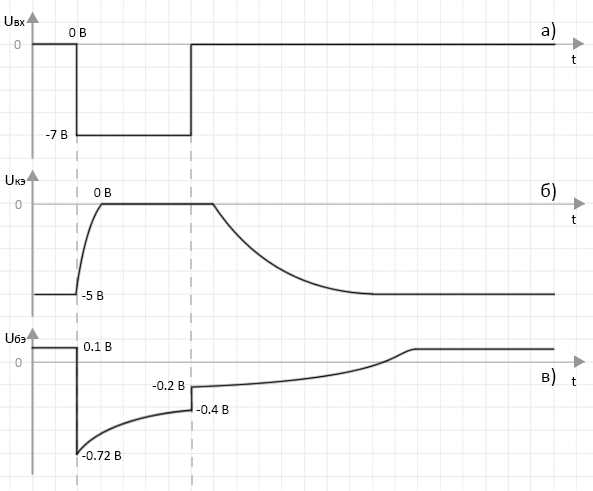
\includegraphics[width=16cm]{img/time}
		\caption{Временные диаграммы: а) б) в)}
		\label{p:2} % название для ссылок внутри кода
	\end{center}
\end{figure}

\begin{table}[H]
	\begin{center}
	\caption{Зависимость $t_\phi$, $t_\text{сп}$, $t_\text{расс}$ от $t_\text{и}$}
		\begin{tabular}{|c|c|c|c|}
		\hline 
		$t_\text{и}$, мкс & $t_\phi$, мкс & $t_\text{сп}$, мкс & $t_\text{расс}$, мкс \\ 
		\hline 
		10 & 3.2 & 25 & 2.6 \\ 
		\hline 
		3 & 2.9 & 25 & 0.2 \\ 
		\hline 
		4 & 3 & 21 & 1.3 \\ 
		\hline 
		6 & 3.1 & 23 & 2.1 \\ 
		\hline 
		8 & 3.2 & 25 & 3 \\ 
		\hline 
		15 & 3.3 & 26 & 2.7 \\ 
		\hline 
		20 & 3.3 & 26 & 2.9 \\ 
		\hline 
		25 & 3.3 & 27 & 3 \\ 
		\hline 
		\end{tabular} 
		\label{tabular:2}
	\end{center}
\end{table}

%TODO график

\begin{table}[H]
	\begin{center}
	\caption{Зависимость $t_\phi$, $t_\text{сп}$, $t_\text{расс}$ от $I_{\text{б}_1}$}
		\begin{tabular}{|c|c|c|c|c|}
		\hline 
		$R$, Ом & $I_{\text{б}_1}$, А & $t_\phi$, мкс & $t_\text{сп}$, мкс & $t_\text{расс}$, мкс \\ 
		\hline 
		680	& 0.004151515 &	1.9 & 20 & 3.8 \\
		\hline
		1000 & 0.003484848 & 3 & 23 & 2.8 \\
		\hline
		1300 &	0,003028327 & 3.2 &	25 & 2.6 \\ 
		\hline
		1630 & 0.002646445 & 4.4 & 26 &	1.5 \\
		\hline
		2000 &	0.002318182 & 6.1 &	26 & 1.1 \\
		\hline
		2330 & 0.002086951 & 8.2 & 27 & 0.3 \\
		\hline
		\end{tabular} 
		\label{tabular:3}
	\end{center}
\end{table}

%TODO график

\begin{table}[H]
	\begin{center}
	\caption{Зависимость $t_\phi$, $t_\text{сп}$, $t_\text{расс}$ от $I_{\text{б}_2}$}
		\begin{tabular}{|c|c|c|c|c|}
		\hline 
		$R_\text{б}$, Ом & $I_{\text{б}_2}$, А & $t_\phi$, мкс & $t_\text{сп}$, мкс & $t_\text{расс}$, мкс \\ 
		\hline 
		120000 & 4.16667E-05 & 3.5 & 22 & 1.7 \\
		\hline
		188000 & 2.65957E-05 & 3.4 & 23 & 2.4 \\
		\hline
		240000 & 2.08333E-05 & 3.2 & 25	& 2.6 \\
		\hline
		308000 & 1.62338E-05 & 3.2 & 27 & 2.6 \\
		\hline
		360000 & 1.38889E-05 & 3.5 & 25 & 2.4 \\
		\hline
		428000 & 1.16822E-05 & 3.3 & 26 & 2.3 \\
		\hline
		\end{tabular} 
		\label{tabular:4}
	\end{center}
\end{table}

%TODO график

\begin{table}[H]
	\begin{center}
	\caption{Зависимость $t_\phi$, $t_\text{сп}$, $t_\text{расс}$ от $I_{\text{кн}}$}
		\begin{tabular}{|c|c|c|c|c|}
		\hline 
		$R_\text{к}$, Ом & $I_{\text{кн}}$, А & $t_\phi$, мкс & $t_\text{сп}$, мкс & $t_\text{расс}$, мкс \\ 
		\hline 
		680 & 0.036764706 & 10 & 29 & 0 \\
		\hline
		1000 & 0.025 & 3.9 & 26 & 2 \\
		\hline
		1160 & 0.021551724 & 3.2 & 25 & 2.6 \\
		\hline
		1330 & 0.018796992 & 2.9 & 24 & 3.6 \\
		\hline
		1680 & 0.014880952 & 2.4 & . & . \\
		\hline
		\end{tabular} 
		\label{tabular:5}
	\end{center}
\end{table}

%TODO график

\section{Выводы}

Полученные экспериментальные зависимости имеют схожий характер изменения с теоретическими. То, что они расположены ниже [на графике], чем теоретические, означает, что реальное значение f транзистора больше, чем указанное в справочнике. 

Таким образом формулы 4.1, 4.2 и 4.3 справедливы.

\end{document}
